%%PREAMBLE %%%%%%%%%%%%%%%%%%%%%%%%%%%%
\documentclass[10pt, a4paper]{article}% size of txt = 10pt
\usepackage[top= 2cm,
			bottom = 2cm,
			left = 1.7cm,
			right = 1.7cm,
			footskip = 0.5cm,
			headsep = 0cm,
			headheight = 0cm
					]{geometry}
\usepackage{amsmath} % math packages
\usepackage{amsfonts}% math packages
\usepackage{amssymb} % math packages
\usepackage{graphicx} %package for including graphics
\usepackage{array}
\usepackage[thinlines]{easytable}
\usepackage{float}
\usepackage[section]{placeins}
\usepackage[hidelinks]{hyperref}
\usepackage[shortlabels]{enumitem}
\usepackage{svg}
\usepackage{bigstrut}
\usepackage{wrapfig,lipsum,booktabs}
\usepackage{subcaption}
\usepackage{xfrac}
\usepackage{pdfpages}
\usepackage{listings}
\usepackage{xcolor}

\usepackage{listings}
\usepackage{color} %red, green, blue, yellow, cyan, magenta, black, white
\definecolor{mygreen}{RGB}{28,172,0} % color values Red, Green, Blue
\definecolor{mylilas}{RGB}{170,55,241}

\definecolor{codegreen}{rgb}{0,0.6,0}
\definecolor{codegray}{rgb}{0.5,0.5,0.5}
\definecolor{codepurple}{rgb}{0.58,0,0.82}
\definecolor{backcolour}{rgb}{1,1,1}

\lstdefinestyle{mystyle}{
    backgroundcolor=\color{backcolour},   
    commentstyle=\color{codegreen},
    keywordstyle=\color{magenta},
    numberstyle=\tiny\color{codegray},
    stringstyle=\color{codepurple},
    basicstyle=\ttfamily\footnotesize,
    breakatwhitespace=false,         
    breaklines=true,                 
    captionpos=b,                    
    keepspaces=true,                 
    numbers=left,                    
    numbersep=5pt,                  
    showspaces=false,                
    showstringspaces=false,
    showtabs=false,                  
    tabsize=2
}
\lstset{style=mystyle}


%date format
\def\mydate{\leavevmode\hbox{\twodigits\day.\twodigits\month.\the\year}}
\def\twodigits#1{\ifnum#1<10 0\fi\the#1}


\usepackage[T1]{fontenc} 
\usepackage{lmodern}
\usepackage{indentfirst}
\setlength{\parindent}{1cm}

\makeatletter
\newcommand{\thickhline}{%
    \noalign {\ifnum 0=`}\fi \hrule height 2pt
    \futurelet \reserved@a \@xhline
}
\newcolumntype{"}{@{\hskip\tabcolsep\vrule width 2pt\hskip\tabcolsep}}
\makeatother
\newcolumntype{?}{!{\vrule width 2pt}}
%%DOC ENVIROMENT%%%%%%%%%%%%%%%%%%%%%%%
\begin{document}
%Title 
\begin{flushleft}%% left justification
	\textbf{\Large{MKC-DVV: Úkol č. 1}}\hfill Filip Paul\\
	\large{Barevné systémy \hfill\mydate}
\end{flushleft}


	\section{\Large Úkol 1:}
	\noindent \textbf{Barevná světla M1,M2 jsou popsána trichomatickými součiniteli v systému CIE RGM následovně:}\\
	$M1: R_{M1} = 10, G_{M1} = 8, B_{M1} = 1$\\
	$M2: R_{M2} = 20, G_{M2} = 5, B_{M2} = 25$\\
	$M = M1 + M2$\\
		\begin{enumerate}
			\item \textbf{Zakreslete všechna světla M1,M2,a M do diagramu CIE x,y.}\\
			Výsledné souřadnice bodů M1,M2 a M byly vypočteny pomocí python scriptu, který je přiložený na konci úkolu. Jedná se vesměs jen o přepis transformačních rovnic
			z prezentace...
			\begin{figure}[ht!]
				\centering
				\includegraphics[width=0.95\textwidth]{CIE_diagram.png}
			\end{figure}
			
			\clearpage
			\item \textbf{Určete vlnovou délku a čistotu (sytost) výsledného světla M. Je vlnová délka výsledného světla M dominantní nebo komplementární?}\\
			Vlnová délka je přibližně 592nm (x = 0.57, y = 0.42) označena bodem D viz. diagram na předchozí straně. Za předpokladu, že referenční bílé světlo W
			má x a y hodnoty 1/3, je vlnová délka dominantní a světlo má sytost $p_e$ cca 0.127.\\\\
			$p_e = \dfrac{WF}{WD} = \dfrac{M_x - W_x}{D_x - W_x} = \dfrac{0.363-0.3333}{0.57 - 0.3333} = 0.127$\\

			\item \textbf{Je také světlo M reprodukovatelné v TV soustavě PAL? Vaší odpověď zdůvodněte jak slovně tak i graficky (pomocí diagramu CIE x,y).}\\
			Z grafu je patrné, že výsledná barva M, vzniklá mísením světel M1 a M2, leží v oblasti pomyslného trojúhelníku, který je vytvořený body R\_PAL,G\_PAL,B\_PAL. Tyto body
			značí základní barvy PAL systému. To znamená, že je výsledná barva M reprodukovatelná systémem PAL.			
			\item \textbf{Výpočty pomocí python scriptu}\\
			\lstinputlisting[language=python]{calc.py}
		\end{enumerate}
		


		\section{\Large Úkol 2:}
		\noindent \textbf{Obrazový signál odpovídající soustavě PAL je digitalizován podle doporučení ITU-R BT.601 ve formátu 4:2:2. Každý vzorek je
		reprezentován 10 bity:}\\
		
		\begin{enumerate}
			\item \textbf{Určete bitovou rychlost nekomprimovaného digitálního signálu. Výsledek vyjádřete v jednotkách bit/s a Mbit/s}\\
			Při všech výpočtech počítám s konvencí, že 1 kbit = 1000 bitů...\\
			Nekomprimovaný signál s formátem 4:2:2 má podle ITU-R BT.601 bitovou rychlost:\\
			Pro 8bit:\\
			$(2\cdot 6.75MHz + 13MHz) \cdot 8bit  = 216Mbit/s $\\
			Pro 10bit:\\
			$(2\cdot 6.75MHz + 13MHz) \cdot 10bit  = 270Mbit/s $\\
			\item \textbf{Určete velikost nekomprimovaného záznamu videosekvence o délce 90 minut. Výsledek vyjádřete v jednotkách bitů (b) 
			a bajtů (B) a gigabajtů (GB)}\\
			Pro 8bit:\\
			$216\,Mbit/s \cdot 90 \cdot 60 = 1166 400 000 000$b = 145800000000\,B = 145.8\,GB\\
			Pro 10bit:\\
			$270\,Mbit/s \cdot 90 \cdot 60 = 1458 400 000 000$b = 182250000000\,B = 182.25\,GB\\

			\item \textbf{Jakého kompresního poměru musí dosáhnout komprimační algoritmus, aby bylo možné uvažovanou videosekvenci uložit na DVD médium
			($4,7\cdot 10^9 B$)?}\\
			Pro 8bit:\\
			$145.8/4.7 = 31.02 \rightarrow$ kompresní poměr musí být alespoň 32:1.\\
			Pro 10bit:\\
			$182.25/4.7 = 38.7 \rightarrow$ kompresní poměr musí být alespoň 32:1.\\


			\item \textbf{Výpočty v bodech 1 až 3 opakujte pro případ, kdy každý vzorek obrazového signálu je reprezentován 8bity. Jaký je procentuální nárůst
			(nebo pokles) bitové rychlost, když každý vzorek je reprezentován 10 bity ?}\\
			Výsledky jsou vepsány do jednotlivých úkolů.\\
			\clearpage
			\item \textbf{Nakreslete závislost velikosti kompresního poměru na délce záznamu videosekvence (formát 4:2:2, 8 a 10 bitů). Uvažujte
			délku videa od 1 až 120 minut, video se má uložit na DVD médium. Jaký je procentuální nárůst (nebo pokles) kompresního poměru pro videosekvenci o délce 120 minut,
			když uvažujeme 10 bitové rozlišení namísto 8bitového ?}\\

			\begin{figure}[ht!]
				\centering
				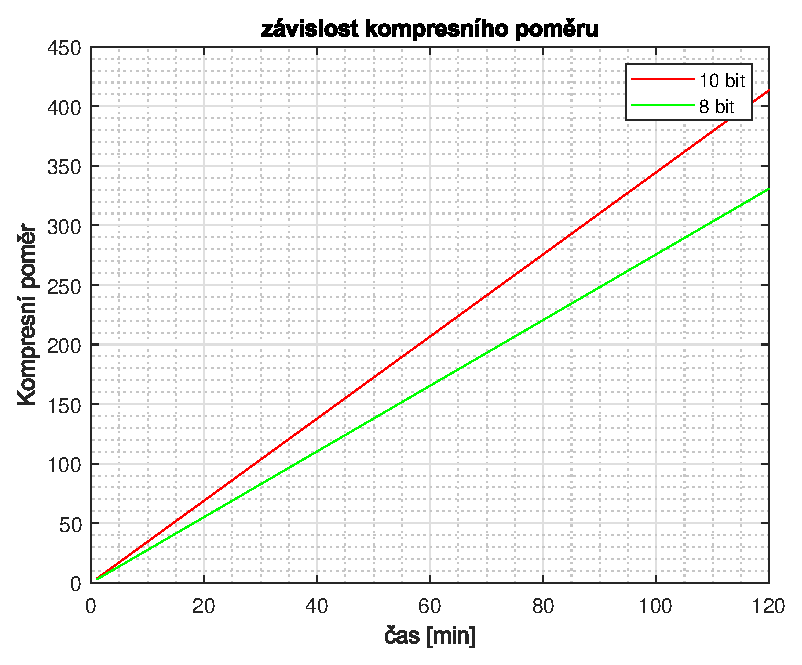
\includegraphics[width=0.8\textwidth]{kompres.eps}
			\end{figure}

			Kompresní poměr v 120 min:\\
			10bit: 413.6170\\
			8bit: 330.8936\\
			nárůst je přibližně 25\%\\
		\end{enumerate}
		
%	\begin{figure}[ht!]
%		\centering
%		\includegraphics[height = 0.80\textheight]{CORDIC_vect_rot.eps}
%		
%	\end{figure}
	

\end{document}

%\[f(x)= (x+2)^2 - \frac{9\cdot 2\pi}{26}\] %%mathematic equatation in display style mode
%%optional:
%	\begin{align} %%this alignes all charakters after & if *is removed equations will be numbered
%	\hspace{5cm}  
%		 x &= a_2 x^2 +_1 x + a_0 \\
% 		x &=x^2 \nonumber		%no number will not add number to eq
%	\end{align}
